\documentclass{eplDoc}



\newcommand{\docType}	{Assignment 4}
\newcommand{\docDate}	{20/04/2012}
\newcommand{\docAuthor}	{gr16 : Mulders Corentin, Pelsser Francois}
\newcommand{\courseCode}{LINGI2365}
\newcommand{\courseName}{Constraint programming}
\usepackage{syntax}

\lstset{breaklines=true, breakatwhitespace=false}

\begin{document}
\maketitle
\newpage

\section{The Brussels airport problem} %6pt

\subsection{Model implementation}
We modelized the problem in comet as a minimization problem with as variables the landing times of the planes and as constraints the fact that all landing times are different and that no landing occurs during a given period depending of the plane after a plane has landed : 
\begin{lstlisting}
range P         = 1..nbPlanes;

range T = (minPTime-maxdelay)..(maxPTime+maxdelay);

var<CP>{int} lTime[P](cp, T);               //actual landing time

minimize<cp>
    sum(p in P)(abs(lTime[p]-prefLTime[p])*delayCost[p])
subject to{
    forall(p1 in P)
    {
        cp.post(abs(lTime[p1] - prefLTime[p1])<maxdelay);
    }
    cp.post(alldifferent(lTime));
    forall(p1 in P, p2 in P: p1 != p2 && p1 > p2)
    {
        cp.post(!(lTime[p1] > lTime[p2]) || (lTime[p1] - lTime[p2]) > indispTime[p1]); 
        cp.post(cp.post(!(lTime[p2] > lTime[p1]) || (lTime[p2] - lTime[p1]) > indispTime[p2]));
    }
}
\end{lstlisting}
\subsection{3 different variable and/or value ordering heuristics}
In all of our three solutions we define a heuristic for ordering the access to the variables representing the planes landing times. The value ordering used for these times is the same in each solution and consist in considering the times closest to the plane's preffered landing time first. 
\subsubsection{First heuristic}
Our first heuristic orders the planes without a defined landing time by the cost of delaying their landing. Since we are dealing with an optimization problem this means that we are more likely to find non-optimal solutions first and those can then be discarded. \\  
Here is what we put in the using part of our comet program to use this heuristic : 
\begin{lstlisting}
forall (p in P: !lTime[p].bound()) by (delayCost[p])
                tryall<cp>(t in T: lTime[p].memberOf(t)) by (abs(t - prefLTime[p]))
                {
                    label(lTime[p], t);
                } 
\end{lstlisting}
\subsubsection{Second heuristic}
The second heuristic orders the planes by the time during which no other plane can land after them. This follows the same logic as the first heuristic as what seems to be more efficient would be to schedule the landing of the planes that cause the greatest loss of time first, which is the opposite. \\ 
Here is what we put in the using part of our comet program to use this heuristic : 
\begin{lstlisting}
forall (p in P: !lTime[p].bound()) by (indispTime[p])
                tryall<cp>(t in T: lTime[p].memberOf(t)) by (abs(t - prefLTime[p]))
                {
                    label(lTime[p], t);
                } 
\end{lstlisting}
\subsubsection{Third heuristic}
Our third heuristic tries to find a landing time for the planes for which the size of the remaining landing time variable domain is the smallest. This allow to reach a solution or a failure more quickly. \\ 
Here is what we put in the using part of our comet program to use this heuristic : 
\begin{lstlisting}
forall (p in P: !lTime[p].bound()) by (lTime[p].getSize())
                tryall<cp>(t in T: lTime[p].memberOf(t)) by (abs(t - prefLTime[p]))
                {
                    label(lTime[p], t);
                } 
\end{lstlisting}

\subsection{Meaningful criterias for comparing different search strategies}

\begin{itemize}
	\item The most basic criteria would simply to consider the execution time of each strategy on the same computer. This allows to roughly assess the quality of the search even though we can't really trust it to be precise since the time could vary from one execution to another. A better solution would be to realise a lot of experiments and use the mean of the times taken. 
	%\item Another straightforward criteria would be the sum of the number of choices and the number of failures. Since the execution time is correlated with this value we would rather use this number of choices and failure instead since it's more reliable. 
	\item Another criteria would be the number of choices which has the advantage of not depending on the cpu load. 
	\item A third criteria similar to the number of choices ois the number of failures, this can show how much search had to be done until an optimal solution was found. 
	
	
\end{itemize}


\subsection{Heuristics comparison} % our heuristics + labelFF
Here are the results of the tests of our different heuristics on the brussels airport file. 
\begin{table}[h]
	\centering
		\begin{tabular}{|c|cccc|}
			\hline
			  & labelFF & first heuristic & second heuristic & third heuristic \\ 
			  \hline
			%\#choices+\#fails  &   236164 & 5475 & 896 & 206 \\ 
			\#choices &  87243 & 689 & 183 & 78 \\ 
			\#fails & 148921 & 4786 & 713 & 128 \\
			time taken[ms] & 37846 & 1124 & 234 & 94 \\ 
			\hline
			
		\end{tabular}
\end{table}
As expected the three criteria are correlated and comparing the heuristics with any of them yields the same results. \\ 
All of our heuristic perform a lot better than labelFF but the second and third are particularly efficient. 

\section{The Knapsack problem}
\subsection{A branch and bound approach} %5pt

\subsubsection{Model description}
In our model we use a boolean variable $x_i$ for each object to represent the fact that the object is placed in the sack or not. We then define the objective function as  $\sum_{i \in N} x_ia_i$ and post a constraint such as $\sum_{i \in N}x_iw_i \le b$. This corresponds to the following in comet : 
\begin{lstlisting}
var<CP>{int} objectsTaken[O](cp, 0..1);         

maximize<cp>
    sum(o in O)(objectsTaken[o]*oUsefullness[o])
subject to{
    cp.post(sum(o in O)(objectsTaken[o]*oWeight[o])<=knapsackCapacity);
}
\end{lstlisting}

\subsubsection{4 different heuristics for variable selection}
\begin{itemize}
	\item \textbf{First heuristic} \\ 
		Our first heuristic consist of starting with the most heavy objects. Thisis a first-fail strategy since this way the sack will be full very quickly : 
		\begin{lstlisting}
            forall (o in O: !objectsTaken[o].bound()) by (-oWeight[o])
                tryall<cp>(v in 0..1: objectsTaken[o].memberOf(v)) by (-v)
                {
                    label(objectsTaken[o], v);
                } 
                
	\item \textbf{Second heuristic} \\ 
		The second heuristic is based on the same idea as the first except now it choses objects that have the lowest $usefullness/weight$ ratio instead. This way we try to start by packing the objects that are both heavy and useless first. \\ 
				Here is what we put in the using part of our comet program to use this heuristic :
		\begin{lstlisting}
	forall (o in O: !objectsTaken[o].bound()) by ((oUsefullness[o]-0.0)/oWeight[o])
                tryall<cp>(v in 0..1: objectsTaken[o].memberOf(v)) by (-v)
                {
                    label(objectsTaken[o], v);
                } 
		\end{lstlisting}
	\item \textbf{Third heuristic} \\ 
	Our third heuristic is naive, it tries to pack the less usefull objects first, the idea being to reach a non-optimal value whenever the sack will be full. However as we will see later this is very unefficient since the maximized sack is not easy to find that way. \\ 
				Here is what we put in the using part of our comet program to use this heuristic :
		\begin{lstlisting}
			forall (o in O: !objectsTaken[o].bound()) by (oUsefullness[o])
                tryall<cp>(v in 0..1: objectsTaken[o].memberOf(v)) by (-v)
                {
                    label(objectsTaken[o], v);
                } 
		\end{lstlisting}
	\item \textbf{Fourth heuristic} \\ 
		Our fourth heuristic is a simple lexicographic one, it simply gets the objects in the same order as they are in the file. \\
				Here is what we put in the using part of our comet program to use this heuristic :
		\begin{lstlisting}
			forall (o in O: !objectsTaken[o].bound()) by (oId[o])
                tryall<cp>(v in 0..1: objectsTaken[o].memberOf(v)) by (-v)
                {
                    label(objectsTaken[o], v);
                } 
		\end{lstlisting}
	
\end{itemize}
\subsubsection{Heuristics tests} %also with labelFF

We measured the performance of our different heuristics by looking at the time taken to find a solution and the total number of failures. Both show the same results so we will only include the graph of the times taken here, the horizontal axis contains the number of the file concerned and the vertical the time taken in milliseconds : 

\begin{center}
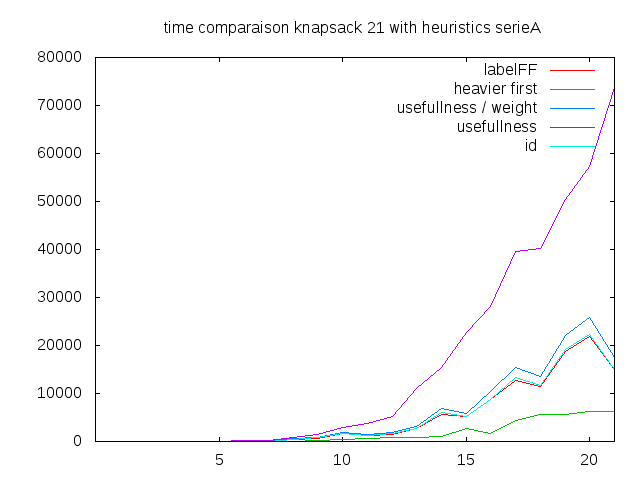
\includegraphics[width=\columnwidth]{q321timeA.png}%
\end{center}

The hierarchy is pretty clear, our first heuristic proves to be the most efficient, followed by the lexicographic and the labelFF. Then comes the second heuristic which is not efficient. \\ 
And worst of all is the third heuristic, his disastrous results can be explained by the fact that in serie A the weights are the same value as the usefullness. In other words when we order by oUsefullness[o] it's as if we ordered by oWeight[o] which is the exact opposite of our best heuristic. 

\subsection{Optimization over iterations} %5pt
\subsubsection{Model}
We represent the problem as a constraint satisfaction problem associated with an upper bound value. We add a totalUsefullness variable to the minimization problem variables. We also use a variable $ub$ which is initialized at the upper bound of the total usefullness of objects in the sack. In the "using" part of our program we force the total usefullness value to be equal to $ub$. Since we want to maximize the totalUSefullness we simply have do decrement the value of $ub$ until we reach a solution and this solution will maximize the total usefullness :  \\  
\begin{lstlisting}
Integer ub;
ub = new Integer(getUB(nbObjects,knapsackCapacity,oWeight, oUsefullness));

var<CP>{int} objectsTaken[O](cp, 0..1);             
var<CP>{int} totalUsefullness(cp, 0..ub);  

whenever cp.getSearchController()@onCompletion(){
    ub := ub-1;
    cp.reStart();
}

whenever cp.getSearchController()@onFeasibleSolution(Solution s){
    cp.exit();
}

solve<cp>
{
    cp.post(sum(o in O)(objectsTaken[o]*oWeight[o])<=knapsackCapacity);
    cp.post(sum(o in O)(objectsTaken[o]*oUsefullness[o]) == totalUsefullness);
}
using{
    cp.post(totalUsefullness == ub);
    [...]
    }
\end{lstlisting}
\subsubsection{Which of the three points must be executed on which events ?}
\begin{itemize}
	\item \textbf{modify the value of ub} : This must be done each time a search finishes with a failure.
	\item \textbf{restart the search} : This must be done after modifying the value of ub to try another search with the new value.
	\item \textbf{end the search} : This is done as soon as a search finishes with a valid solution.
\end{itemize}

\subsubsection{How is the value of ub modified to be sure to find the optimal solution ?}
Since the totaUsefullness value is a sum of integers it is discrete so we can modify the value of ub by substracting 1 from it at each iteration. \\ 
This guarantees to find an optimal solution because the value of ub is initialized at the upper bound of the totalUsefullness and then it is lowered without skipping any interesting value s the first valid solution achieved will be the one with the highest possible totalUsefullness. 

\subsubsection{Why initialize ub with the upper bound ?}
Because we want to maximize the totalUsefullness, starting with the upper bound and gradually reducing the value of ub allows to stop at the first valid solution found. This solution will be the one with the highest totalUsefullness among the solution that satisfy the constraints. \\ 
On the opposite, if we had wanted to minimize the objective we would have initialized it with the lower bound and then incremented it.

\subsubsection{Experiments on knapsack-A and knapsack-B}
%todo


\subsection{Optimization via divide and conquer} %4pt
\subsubsection{Which of the four points must be executed on which events ?}
We know that the maximum is between 2 bounds.  We divide this bonded space in two and try to find if there is a solution in the part with the bigger values.  If there is no solution we are sure than the maximum we are looking after is in the half with smaller values so we have to update the upper bound (ii is in onCompletion).  If a solution is found, we are sure that the maximum we search is bigger or equal to this solution, so we update the lower bound (i is in onFeasibleSolution). We restart after each update (lb or ub) and we stop when we find a solution equals to the upper bound (we are sure that there cannot exist a bigger solution).\\
%We are using ceil instead of floor because we could be blocked with floor.  For instance if there is a solution at the objective function with the objective a and the solution we search is with objective a+1, we will find the solution with a and update lb to a, we will then still find the solution with objective a because the interval will be $\left[ \frac{a+a+1}2 ; a+1 \right]$ wich is equal to $\left[ a ; a+1 \right]$ so we are in an infinite loop.  If, instead, we set the 
\subsubsection{Experiments on knapsack-A, knapsack-B and knapsack-C}



\end{document}
